\documentclass[10pt,letterpaper]{article}

\usepackage[margin=1in]{geometry}
\usepackage{iftex}
% mathptmx has no TU-encoded faces, so under XeTeX (Tectonic) earlier versions fell back
% to Latin Modern regular and lost every bold and italic. Use Termes there.
\ifPDFTeX\usepackage{mathptmx}\else\usepackage{fontspec}\setmainfont{texgyretermes}[Extension=.otf,UprightFont=*-regular,BoldFont=*-bold,ItalicFont=*-italic,BoldItalicFont=*-bolditalic]\fi
\usepackage{amsmath}
\usepackage{amssymb}
\usepackage{graphicx}
\usepackage{booktabs}
\usepackage{listings}
\usepackage{xcolor}
\usepackage{tikz}
\usetikzlibrary{positioning,arrows.meta,fit,backgrounds,calc}
\usepackage{natbib}
\usepackage[colorlinks=true,linkcolor=blue,citecolor=blue,urlcolor=blue]{hyperref}
\usepackage{microtype}
\usepackage{parskip}
\usepackage{titlesec}
\usepackage{enumitem}
\usepackage{caption}

\setlength{\parskip}{6pt}
\setlength{\parindent}{0pt}
\setlength{\emergencystretch}{3em}

\lstset{
  basicstyle=\small\ttfamily,
  breaklines=true,
  frame=single,
  numbers=left,
  numberstyle=\tiny,
  xleftmargin=2em,
  framexleftmargin=1.5em,
  backgroundcolor=\color{gray!8},
}

\title{\textbf{Agent Manifest: Portable, Hardware-Attestable Identity and
Provenance for AI Agents}}

\author{
  Imran Siddique \\
  OPAQUE Systems \\[4pt]
  \normalsize \url{https://github.com/agentrust-io/agent-manifest}
}

\date{October 1, 2026 \\ \small Technical report, version 2}

\begin{document}

\maketitle

\begin{abstract}
Agent Manifest proposes a signed record of the artifacts that define
an AI agent, including its system prompt, model, policy, tools, retrieval corpus,
memory, decision trace, delegation, supply chain, and human approvals. Artifact
digests and canonical serialization make changes to the recorded baseline
detectable when a verifier has the relevant artifacts and trusted keys. The
design composes SPIFFE identities, RFC 8785 canonicalization, Ed25519 signatures,
an optional ML-DSA-65 profile, and hardware-attestation bindings. This technical
report describes the original model and preserves the recorded Ed25519 software
benchmarks, delegation checks, and tamper probes. Signed metadata alone does not
prove that the recorded configuration was used during execution. The evaluation
does not measure post-quantum performance or establish live hardware provenance;
continuous verification of mutable memory and retrieval state is outside its
scope. Current SDK behavior and normative requirements are maintained separately.
\end{abstract}

\paragraph{Scope of this edition.}
This is an author-prepared technical report, not peer reviewed and not a
normative specification. It revises a manuscript originally dated June 23, 2026;
the recorded experiments include later runs and have not been rerun for this
edition. Architectural requirements describe intended checks, not proof that
the historical SDK implements every check. Consult the linked project
specification and limitations before implementing the design.
Version 2 (October 1, 2026) corrects the signature pre-image description, the tamper-probe field
list, the delegation per-hop figure and the conformance test count, states the
inferred SDK revision, records that the evaluated verifier did not authenticate
human approvals, adds the result of an October 2026 rerun, replaces two
repository citations with the published reports, and restores bold and italic
type that the Tectonic build had dropped; the recorded numbers are unchanged.

\noindent\textbf{Patent Pending.}

\tableofcontents
\newpage

\section{Introduction}
\label{sec:intro}

An AI agent is not a single artifact. What it does is determined by a system prompt,
a policy bundle, a set of tool schemas, a model and its version, a retrieval corpus,
a memory state, the decisions it records, the sub-agents it delegates to, its supply
chain, and the human approvals that gate its actions. Today none of these is
attested. A signed JWT proves which credential called an API; it proves nothing about
the agent behind the call.

This is the \emph{agent identity gap}. When an agent acts in a regulated environment,
its operator can show policy documents, SOC reports, and mutable application logs,
none of which prove what actually ran. A reviewer cannot confirm which system prompt
defined the agent, which model version executed, which policy was in force, which
tools were authorized, whether the retrieval corpus or memory was poisoned, what the
agent decided, whether a human approved a high-risk action, or whether the deployed
binary matches the one reviewed.

Agent Manifest closes this gap. It binds the artifacts that define an agent into one
cryptographically signed, hardware-attestable, tamper-evident record. Its central
design choice is \emph{tamper-evidence over tamper-resistance}: rather than trying to
prevent change, the manifest makes change \emph{detectable} by any third party that
holds it and compares it to hardware attestation. Each artifact is bound by hash;
the manifest is canonicalized with RFC~8785~\citep{jcs8785}, signed with
Ed25519~\citep{eddsa8032} (or post-quantum ML-DSA-65~\citep{mldsa204}), and registered
on an append-only transparency log.

\subsection*{The ten unattested surfaces}

Agent Manifest binds ten artifacts: (1)~the system prompt, (2)~the policy bundle,
(3)~the tool manifest, (4)~the model identity, (5)~the retrieval (RAG) corpus,
(6)~the memory baseline, (7)~the decision trace, (8)~the A2A delegation chain,
(9)~the supply chain, and (10)~the human-in-the-loop approvals. Each is a surface an
adversary can alter without detection in today's deployments; each becomes
tamper-evident once bound (Section~\ref{sec:model}).

\subsection*{Contributions}

\begin{itemize}[leftmargin=1.5em]
  \item \textbf{A manifest schema} binding ten agent-defining artifacts, with a
    SPIFFE identity and a confirmation key (Section~\ref{sec:model}).
  \item \textbf{Cryptographic protocols}: RFC~8785 canonicalization, Ed25519 and a
    post-quantum ML-DSA-65 profile, and RFC~9162 Merkle commitments
    (Section~\ref{sec:crypto}).
  \item \textbf{A fail-closed verification protocol} with explicit result states and
    revocation (Section~\ref{sec:verification}).
  \item \textbf{Delegation and human-oversight} bindings that prevent scope laundering
    across agent hops (Section~\ref{sec:deleg}).
  \item \textbf{Integration and conformance}: composition with cMCP, TRACE, and
    AGT (Section~\ref{sec:integration}), and an open SDK with a conformance specification
    of 197 tests across four levels (Section~\ref{sec:conformance}).
\end{itemize}

\subsection*{Paper structure}

Section~\ref{sec:background} reviews the primitives Agent Manifest composes.
Section~\ref{sec:model} defines the manifest. Section~\ref{sec:crypto} gives the
cryptographic protocols and Section~\ref{sec:verification} the verification protocol.
Section~\ref{sec:deleg} covers delegation and human oversight,
Section~\ref{sec:integration} integration with the surrounding stack,
Section~\ref{sec:conformance} conformance, Section~\ref{sec:related} related work and
regulatory mapping, and Section~\ref{sec:conclusion} concludes.

\section{Background}
\label{sec:background}

Agent Manifest composes established primitives rather than inventing new ones.

\paragraph{Workload identity.}
SPIFFE~\citep{spiffe2018} gives workloads cryptographic identities of the form
\texttt{spiffe://trust-domain/path}. Agent Manifest uses SPIFFE URIs as the canonical
form for both \texttt{agent\_id} (the agent) and \texttt{issuer} (the signing
authority), reusing identity already issued by SPIRE, Kubernetes, and service meshes
without a new registry. Human approvers, who are not workloads, are named instead by
OIDC subject, \texttt{mailto:} URI, or W3C DID.

\paragraph{Attestation.}
The manifest's hardware evidence follows RATS~\citep{rats2021} and normalizes
platform reports through EAT~\citep{eat2023}. A TEE attestation report binds the
manifest's signing key to a measured environment, so a verifier can confirm the
manifest was produced where it claims.

\paragraph{Canonicalization and signatures.}
Every signature is computed over the RFC~8785 JSON Canonicalization Scheme
(JCS)~\citep{jcs8785} form of the signed fields, so independent implementations
produce byte-identical pre-images. Signatures use Ed25519~\citep{eddsa8032} in the
standard profile and ML-DSA-65~\citep{mldsa204} in the post-quantum profile.

\paragraph{Tamper-evident logs.}
Artifact collections (the retrieval corpus, the decision trace) and the transparency
anchor use Merkle trees with RFC~9162~\citep{ct9162} domain-separated interior nodes;
transparency-log entries follow the Sigstore/Rekor model~\citep{sigstore2021}.
Identifiers are time-ordered UUIDv7~\citep{uuid9562}.

\paragraph{Relationship to the runtime stack.}
Agent Manifest answers \emph{who and what} an agent is. It is complementary to
cMCP~\citep{cmcp2026}, which enforces policy and produces hardware-attested evidence
at the tool-call boundary, and to TRACE~\citep{trace2026}, the portable evidence
format cMCP emits; the manifest's decision-trace artifact references a TRACE
audit chain. It composes with the Agent Governance Toolkit (AGT)~\citep{agt2026},
which supplies policy enforcement, trust scoring, and observability: the manifest's
attestation level feeds AGT's trust score, its delegation chain feeds scope-narrowing
policy, and its revocation feeds AGT's kill switch.

\section{The Manifest}
\label{sec:model}

A manifest is a JSON document with a canonical (RFC~8785) serialization over which a
signature is computed. Table~\ref{tab:top} lists the top-level fields.

\begin{table}[h]
\centering
\small
\caption{Top-level manifest fields (optional fields italicized).}
\label{tab:top}
\begin{tabular}{p{3.7cm}p{3.6cm}p{4.9cm}}
\toprule
Field & Type & Notes \\
\midrule
\texttt{manifest\_id} & UUIDv7~\citep{uuid9562} & time-ordered unique id \\
\texttt{agent\_id} & SPIFFE URI & the agent workload \\
\texttt{version} & string & schema version (\texttt{0.1}) \\
\texttt{issued\_at} & ISO 8601 UTC & issuance time \\
\texttt{expires\_at} & ISO 8601 UTC & $\geq$ 1\,h after, $\leq$ 365\,days \\
\texttt{issuer} & SPIFFE URI & signing authority \\
\texttt{crypto\_profile} & \texttt{standard} $|$ \texttt{post-quantum} & signature suite \\
\texttt{artifacts} & object & the ten artifact bindings (Table~\ref{tab:artifacts}) \\
\texttt{attestation} & object & TEE evidence; required at Level~1+ \\
\emph{\texttt{delegation\_chain}} & list & present when the agent was delegated to \\
\emph{\texttt{hitl\_record}} & object & present when policy mandates human approval \\
\texttt{signature} & object & algorithm, key id, signed-field list, value \\
\emph{\texttt{transparency\_log\_entry}} & object & inclusion proof; required in production \\
\bottomrule
\end{tabular}
\end{table}

\subsection{The ten artifact bindings}

The \texttt{artifacts} object binds each agent-defining surface by hash and metadata,
so any post-approval change to the underlying artifact is detectable.
Table~\ref{tab:artifacts} summarizes the bindings.

\begin{table}[h]
\centering
\small
\caption{The ten artifact bindings and their key bound fields.}
\label{tab:artifacts}
\begin{tabular}{p{0.4cm}p{3.0cm}p{8.6cm}}
\toprule
\# & Binding & Key bound fields \\
\midrule
1 & System prompt & \texttt{hash}, version, classification, safety level \\
2 & Policy bundle & \texttt{hash}, policy language (Cedar/Rego/YAML/composite), enforcement mode, AGT version \\
3 & Tool manifest & \texttt{catalog\_hash}, per-tool entries, dynamic-registration and rug-pull policy \\
4 & Model identity & provider, model id, version, deployment type, \texttt{model\_hash}, attestation type \\
5 & RAG corpus & \texttt{merkle\_root}, document count, ingestion-policy hash, poisoning scan \\
6 & Memory baseline & \texttt{snapshot\_hash}, memory type, drift policy, TTL \\
7 & Decision trace & \texttt{audit\_chain\_root} (a TRACE chain), trace type, signing key id, entry count \\
8 & Delegation chain & per-hop principal, \texttt{scope\_grant}, delegation signature, principal manifest id \\
9 & Supply chain & container/base-image digests, SLSA provenance, SBOM, MCP servers \\
10 & Human-in-the-loop & required flag, approvals, escalation policy \\
\bottomrule
\end{tabular}
\end{table}

Figure~\ref{fig:binding} shows the binding structure: ten heterogeneous artifacts
each reduce to a digest, the digests collect into the \texttt{artifacts} object,
the whole document is serialized with RFC~8785 canonical JSON, and one signature
plus an optional transparency-log inclusion proof close the record. Any change to
any bound artifact changes its digest, changes the canonical bytes, and invalidates
the single signature: this is what makes the record tamper-evident.

\begin{figure}[h]
\centering
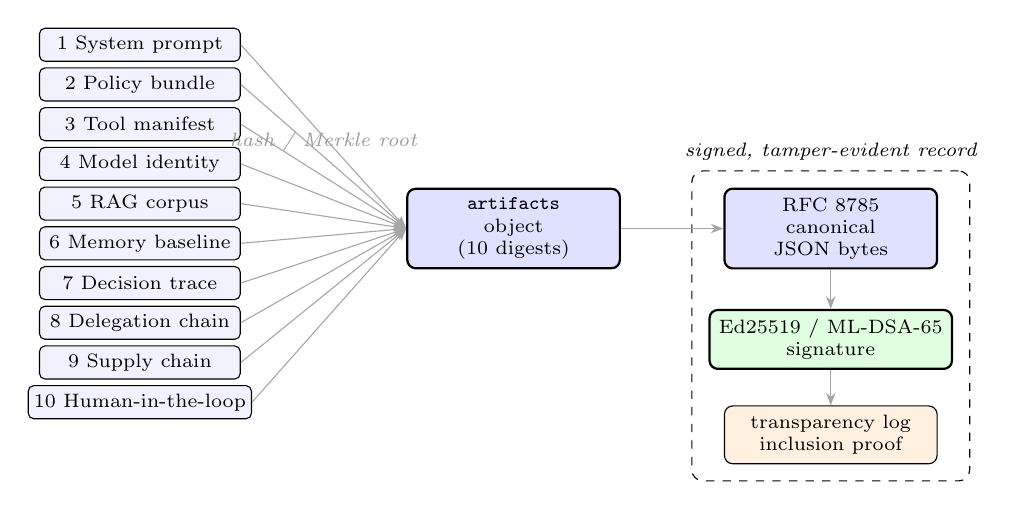
\begin{tikzpicture}[
  font=\scriptsize,
  art/.style={draw, rounded corners=2pt, minimum width=2.55cm, minimum height=0.42cm,
    fill=blue!5, align=left, inner sep=2pt},
  core/.style={draw, thick, rounded corners=3pt, minimum width=2.7cm, minimum height=0.9cm,
    fill=blue!12, align=center},
  sig/.style={draw, thick, rounded corners=3pt, minimum width=2.7cm, minimum height=0.7cm,
    fill=green!12, align=center},
  tl/.style={draw, rounded corners=3pt, minimum width=2.7cm, minimum height=0.65cm,
    fill=orange!12, align=center},
  ln/.style={-{Stealth[length=1.6mm]}, gray!70},
]
% Left column: ten artifact bindings
\node[art] (a1)  {1 System prompt};
\node[art] (a2)  [below=2pt of a1] {2 Policy bundle};
\node[art] (a3)  [below=2pt of a2] {3 Tool manifest};
\node[art] (a4)  [below=2pt of a3] {4 Model identity};
\node[art] (a5)  [below=2pt of a4] {5 RAG corpus};
\node[art] (a6)  [below=2pt of a5] {6 Memory baseline};
\node[art] (a7)  [below=2pt of a6] {7 Decision trace};
\node[art] (a8)  [below=2pt of a7] {8 Delegation chain};
\node[art] (a9)  [below=2pt of a8] {9 Supply chain};
\node[art] (a10) [below=2pt of a9] {10 Human-in-the-loop};

% Middle: the artifacts object (collected digests)
\node[core] (obj) [right=2.1cm of a5, yshift=-9pt] {\texttt{artifacts}\\object\\(10 digests)};

% edges from each artifact to the object, labeled as a digest
\foreach \n in {a1,a2,a3,a4,a5,a6,a7,a8,a9,a10} {
  \draw[ln] (\n.east) -- (obj.west);
}
\node[gray!80] at ($(a5.east)!0.5!(obj.west) + (0,0.95)$) {\itshape hash / Merkle root};

% Right: canonicalize -> sign -> transparency log
\node[core] (canon) [right=1.3cm of obj] {RFC~8785\\canonical\\JSON bytes};
\node[sig]  (sign)  [below=0.5cm of canon] {Ed25519 / ML-DSA-65\\signature};
\node[tl]   (tlog)  [below=0.45cm of sign] {transparency log\\inclusion proof};

\draw[ln] (obj.east) -- (canon.west);
\draw[ln] (canon.south) -- (sign.north);
\draw[ln] (sign.south) -- (tlog.north);

% background box around the signed record
\begin{scope}[on background layer]
  \node[draw, dashed, rounded corners, fit=(canon)(sign)(tlog), inner sep=6pt,
        label={[font=\scriptsize\itshape]above:signed, tamper-evident record}] {};
\end{scope}
\end{tikzpicture}
\caption{Ten agent-defining artifacts each reduce to a digest, collect into the
\texttt{artifacts} object, canonicalize under RFC~8785, and are closed by one
signature and an optional transparency-log inclusion proof. Any post-approval change
to any artifact changes its digest and invalidates the single signature.}
\label{fig:binding}
\end{figure}

The binding pattern is uniform: each artifact contributes a digest (a SHA-256 hash, a
Merkle root for collections, or an audit-chain root for the decision trace) into the
signed manifest, so verifying the signature plus recomputing the artifact's digest
detects any divergence. The model-identity binding distinguishes a \emph{hash-bound}
model (weights digest verifiable) from a \emph{provider-asserted} one (a hosted API,
where the provider's assertion is the strongest available evidence). The
decision-trace binding is the join point with the runtime stack: its
\texttt{audit\_chain\_root} is the root of the TRACE audit chain cMCP
produces~\citep{trace2026,cmcp2026}.

\section{Cryptographic Protocols}
\label{sec:crypto}

\subsection{Canonicalization and signing}

The signature pre-image is the RFC~8785 JCS~\citep{jcs8785} serialization of the
manifest's signed fields, encoded as UTF-8 without a BOM; Ed25519 and ML-DSA-65 sign
these bytes directly. SHA-256 (SHAKE-256 in the post-quantum profile) is the
artifact-digest and Merkle hash. JCS is required precisely
because ad-hoc sorting diverges on non-ASCII strings and IEEE~754 numbers; two
conformant implementations must produce identical bytes.

The standard profile signs with Ed25519~\citep{eddsa8032}; the post-quantum profile
signs with ML-DSA-65 (NIST FIPS~204)~\citep{mldsa204}; the hybrid mode carries both a
classical and a post-quantum signature over the \emph{identical} pre-image, and a
verifier requires both to validate. A key id is the SHA-256 hex digest of the raw
public-key bytes, and signature values are base64url without padding. The signature
block records its \texttt{algorithm}, \texttt{key\_id}, \texttt{key\_type}
(\texttt{software} $|$ \texttt{hsm} $|$ \texttt{tee-sealed}), and the explicit list of
\texttt{signed\_fields}.

\subsection{Merkle commitments}

Artifact collections commit via Merkle trees with RFC~9162~\citep{ct9162}
domain-separated nodes (leaf $0x00$, interior $0x01 \,\|\, \text{left} \,\|\,
\text{right}$), so the retrieval corpus binds as a single \texttt{merkle\_root} over
its documents and the transparency-log entry carries an RFC~9162 inclusion proof. The
decision trace binds as a hash-chained or Merkle-log audit root.

\subsection{Post-quantum profile}

Because manifests may need to remain verifiable for years, Agent Manifest specifies a
post-quantum profile from v0.1: \texttt{crypto\_profile: post-quantum} selects
ML-DSA-65 and SHAKE-256, and the hybrid mode lets a deployment carry both classical
and post-quantum signatures during migration, so a manifest stays verifiable whether
or not a verifier has post-quantum support.

\section{Verification}
\label{sec:verification}

\subsection{Signed fields}

A fixed, normative set of fields is covered by the signature: the manifest metadata
(\texttt{manifest\_id}, \texttt{agent\_id}, \texttt{version}, \texttt{issued\_at},
\texttt{expires\_at}, \texttt{issuer}, \texttt{crypto\_profile}), the
\texttt{artifacts}, the \texttt{delegation\_chain}, and the \texttt{hitl\_record},
among others. Three fields are deliberately \emph{outside} the signature because they
are appended after signing: the \texttt{attestation} report (bound instead through the
key the report attests), the \texttt{signature} block itself, and the
\texttt{transparency\_log\_entry} (which can only exist after the signed manifest is
registered). Within \texttt{hitl\_record}, the \texttt{approvals} list is normalized
to empty before signing, so approvals attach after issuance and each must be
authenticated by its own \texttt{approval\_signature}.

\subsection{Fail-closed semantics}

Verification is fail-closed: \texttt{VALID} requires a verifiable signature against a
trusted key. A signed manifest whose key is not trusted returns
\texttt{UNVERIFIABLE}; an unsigned manifest returns \texttt{SIGNATURE\_MISSING};
neither returns \texttt{VALID}. The verifier emits a structured result: an overall
state (\texttt{VALID}, \texttt{MISMATCH}, \texttt{EXPIRED}, \texttt{REVOKED},
\texttt{INCOMPLETE}, \texttt{ATTESTATION\_UNAVAILABLE}, \texttt{INCOMPATIBLE\_VERSION},
\texttt{SIGNATURE\_MISSING}, or \texttt{UNVERIFIABLE}) plus per-artifact field
results (\texttt{MATCH}, \texttt{MISMATCH}, \texttt{NOT\_BOUND}, \texttt{EXPIRED}) and,
where present, delegation and HITL results. A verifier checks \texttt{version} before
anything else: an unsupported version returns \texttt{INCOMPATIBLE\_VERSION}, never
\texttt{VALID}.

\subsection{Revocation}

A manifest can be revoked before \texttt{expires\_at} (for a leaked key, a
withdrawn approval, or a compromised artifact). Revocation records are signed and
distributed as an append-only, JSON-lines certificate revocation list; a verifier
consults current revocation state at verification time and returns \texttt{REVOKED}
for a listed manifest. Revocation also drives the downstream kill switch when Agent
Manifest is paired with AGT (Section~\ref{sec:integration}).

\section{Delegation and Human Oversight}
\label{sec:deleg}

\subsection{Delegation chains}

When one agent delegates to another (an A2A hop), the sub-agent's manifest carries a
\texttt{delegation\_chain}: an ordered list of hops, each naming the delegating
principal, a \texttt{scope\_grant} (the tools and data classifications the hop is
permitted), a delegation signature, and the principal's manifest id and attestation
hash. Because each hop is signed and references the parent manifest, a verifier
reconstructs the full chain of authority from the leaf agent back to the root.

The chain enforces \emph{monotonic narrowing}: a hop's scope must be a subset of the
scope it was granted, so a sub-agent cannot acquire capabilities its delegator lacked:
the \emph{scope-laundering} attack. A maximum delegation depth (default~3) bounds
the chain and prevents unbounded re-delegation. The delegation chain is the input AGT
uses to apply scope-narrowing policy at runtime (Section~\ref{sec:integration}).
Figure~\ref{fig:delegation} shows a three-principal chain and the capability set
shrinking at each hop.

\begin{figure}[h]
\centering
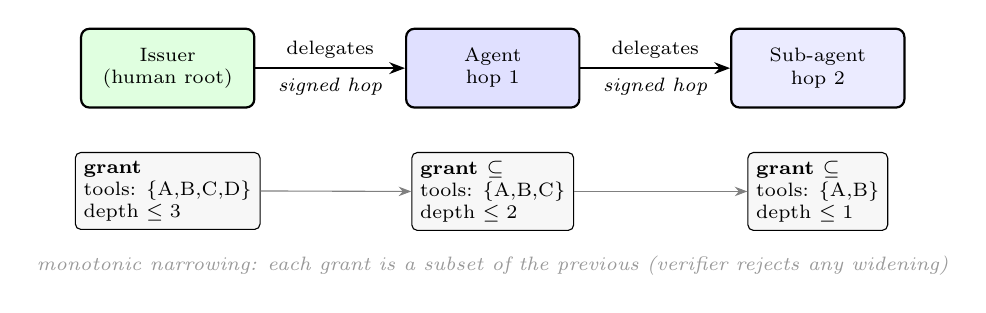
\begin{tikzpicture}[
  font=\scriptsize,
  node distance=1.9cm,
  princ/.style={draw, thick, rounded corners=3pt, minimum width=2.2cm,
    minimum height=1.0cm, align=center},
  scope/.style={draw, rounded corners=2pt, fill=gray!6, align=left, inner sep=3pt,
    font=\scriptsize},
  hop/.style={-{Stealth[length=2mm]}, thick},
]
\node[princ, fill=green!12] (iss)  {Issuer\\{\scriptsize (human root)}};
\node[princ, fill=blue!12]  (ag)   [right=of iss] {Agent\\{\scriptsize hop~1}};
\node[princ, fill=blue!8]   (sub)  [right=of ag]  {Sub-agent\\{\scriptsize hop~2}};

\draw[hop] (iss) -- node[above, font=\scriptsize]{delegates} node[below, font=\scriptsize\itshape]{signed hop} (ag);
\draw[hop] (ag)  -- node[above, font=\scriptsize]{delegates} node[below, font=\scriptsize\itshape]{signed hop} (sub);

\node[scope] (s0) [below=0.55cm of iss] {\textbf{grant}\\tools: \{A,B,C,D\}\\depth $\leq 3$};
\node[scope] (s1) [below=0.55cm of ag]  {\textbf{grant $\subseteq$}\\tools: \{A,B,C\}\\depth $\leq 2$};
\node[scope] (s2) [below=0.55cm of sub] {\textbf{grant $\subseteq$}\\tools: \{A,B\}\\depth $\leq 1$};

\draw[-{Stealth[length=1.6mm]}, gray] (s0.east) -- (s1.west);
\draw[-{Stealth[length=1.6mm]}, gray] (s1.east) -- (s2.west);

\node[gray!80, font=\scriptsize\itshape] at ($(s0.south)!0.5!(s2.south) + (0,-0.45)$)
  {monotonic narrowing: each grant is a subset of the previous (verifier rejects any widening)};
\end{tikzpicture}
\caption{Delegation chain from issuer to agent to sub-agent. Each hop is signed by the
delegating principal and references the parent manifest; the capability grant narrows
monotonically (tools drop, depth budget decrements). The verifier rejects any hop whose
scope exceeds its delegator's grant, defeating scope laundering.}
\label{fig:delegation}
\end{figure}

\subsection{Human-in-the-loop approvals}

When policy requires a human to authorize an action, the manifest carries an
\texttt{hitl\_record}: the requirement flag, the approvals collected, and an
escalation policy. Each approval names the approver (by OIDC subject,
\texttt{mailto:} URI, or DID, not a SPIFFE workload identity, since the approver is
a person), the approved scope (a risk tier and the artifact set the human signed off
on), and a timestamp. A verifier returns \texttt{APPROVED}, \texttt{EXPIRED},
\texttt{NOT\_REQUIRED}, \texttt{MISSING}, or \texttt{APPROVAL\_INSUFFICIENT}. When
each approval's signature is verified against the approver's key, an auditor has
evidence that an identified human approved the recorded scope, which supports
human-oversight obligations such as EU AI Act Article~14~\citep{euaiact2024}. At the
evaluated SDK revision, \texttt{verify\_manifest} did not check
\texttt{approval\_signature}: a signed manifest whose approvals were replaced with
forged ones still returned \texttt{VALID} and \texttt{APPROVED}
(\texttt{experiments/results/rerun-2026-10-01}). The SDK has verified approval
signatures in that path since commit 36d0c89 (August 22, 2026).

\section{Integration}
\label{sec:integration}

Agent Manifest is deliberately one layer of a stack. It answers \emph{identity and
provenance}; three neighboring systems answer the rest.

\paragraph{cMCP: runtime attestation.}
cMCP~\citep{cmcp2026} is the reference runtime that enforces the manifest's policy and
tool bindings at the Model Context Protocol boundary. It detects tool-catalog
``rug-pulls'' before the agent sees the change, and it signs a decision record per
tool call. The manifest's decision-trace artifact (Table~\ref{tab:artifacts},~\#7)
binds the root of the audit chain cMCP produces, so a verifier can tie the static
manifest to the dynamic record of what the agent did.

\paragraph{TRACE: portable evidence.}
TRACE~\citep{trace2026} is the portable, hardware-attested evidence format cMCP emits
for each session. Where the manifest establishes the agent at deployment time, a TRACE
Trust Record attests its behavior at run time; the two are joined by the manifest's
\texttt{audit\_chain\_root}, which is the same chain TRACE commits.

\paragraph{AGT: policy and observability.}
The Agent Governance Toolkit~\citep{agt2026} consumes the manifest at runtime: the
attestation level feeds AGT's trust score, the delegation chain feeds scope-narrowing
policy, the decision-trace root feeds AGT's governance event sink, and a revocation
record triggers AGT's kill switch. Agent Manifest supplies the verifiable facts; AGT
acts on them.

\paragraph{MCP and A2A.}
The tool-manifest binding extends the MCP~\citep{mcp2024} initialize handshake with a
pinned catalog hash, and the delegation chain proposes an A2A delegation format. Both
are protocol-agnostic; MCP is the reference surface.

\section{Conformance and Reproducibility}
\label{sec:conformance}

Agent Manifest is realized by an open-source Python SDK (\texttt{agent-manifest}) and
a formal conformance suite. The SDK provides the data model, signing
(\texttt{generate\_ed25519}, signers/verifiers), verification
(\texttt{verify\_manifest}), canonicalization, Merkle construction, delegation and
revocation, hardware-attestation providers (TPM, SEV-SNP, TDX, OPAQUE) with
auto-selection, and a \texttt{manifest} CLI (\texttt{keygen}, \texttt{create},
\texttt{sign}, \texttt{attest}, \texttt{verify}, \texttt{revoke}).

\subsection{Conformance levels}

Conformance is defined at four assurance levels, each adding evidence
(Table~\ref{tab:levels}). A claim of conformance is checked, not asserted. The suite
runs against versioned example manifests: software-only, TPM-attested, a fully
populated ten-artifact manifest, multi-hop delegation chains, a HITL manifest, and a
revocation record.

\begin{table}[h]
\centering
\small
\caption{Agent Manifest conformance levels.}
\label{tab:levels}
\begin{tabular}{cll}
\toprule
Level & Adds & Use case \\
\midrule
0 & signature + binding validation (software keys) & development and staging \\
1 & TPM attestation & production with a TPM root of trust \\
2 & SEV-SNP / TDX attestation & confidential-VM deployments \\
3 & post-quantum (ML-DSA-65) signatures & long-lived / PQ-required records \\
\bottomrule
\end{tabular}
\end{table}

\subsection{Conformance modules}

The specification defines 197 conformance tests across five modules
(Table~\ref{tab:modules}). At the evaluated SDK revision the five corresponding test
files contain 191 tests (\texttt{AM-BIND} 44, \texttt{AM-CRYPTO} 29,
\texttt{AM-ATTEST} 38, \texttt{AM-VERIFY} 49, \texttt{AM-COMPAT} 31; four
post-quantum tests skip without the ML-DSA dependency), within an SDK suite of 558
tests covering binding, canonicalization, signing, attestation, delegation, HITL,
revocation, transparency, Merkle construction, and corpus poisoning detection.

\begin{table}[h]
\centering
\small
\caption{Conformance modules and the test counts the specification defines (197 total).}
\label{tab:modules}
\begin{tabular}{llr}
\toprule
Module & Validates & Tests \\
\midrule
\texttt{AM-BIND} & artifact binding, hashing, Merkle trees & 47 \\
\texttt{AM-CRYPTO} & signatures and RFC~8785 canonicalization & 38 \\
\texttt{AM-ATTEST} & TEE attestation binding and field cross-checks & 29 \\
\texttt{AM-VERIFY} & verification, mismatch, delegation, revocation & 52 \\
\texttt{AM-COMPAT} & AGT, cMCP, and MCP integration & 31 \\
\midrule
\textbf{Total} & & \textbf{197} \\
\bottomrule
\end{tabular}
\end{table}

\subsection{Evaluation}
\label{sec:eval}

We measured signing and verification cost, on-the-wire size, delegation-chain
scaling, and tamper detection with a deterministic harness
(\texttt{experiments/bench.py}) that drives the shipped SDK directly. The manifests
timed are the SDK's own committed example manifests (loaded, stripped of their
placeholder signatures, re-signed with a fresh key, and confirmed to verify
\texttt{VALID} before timing) so every input is schema-valid under the shipped
Pydantic models and no manifest body is hand-authored. All numbers below are
medians over 2000 iterations (1000 for delegation chains) after 50 warmup
iterations, on Python~3.12, Windows~11, ARMv8 (Qualcomm). The SDK revision was not
recorded; the inferred revision is agent-manifest 67c21db, whose SDK source and
examples match tag \texttt{python-v0.2.0}. Only the Ed25519
\emph{standard} profile is measured: the post-quantum ML-DSA-65 profile requires
Open Quantum Safe bindings (\texttt{import oqs}), which are not installed in this
environment, and the SDK's \texttt{pq} extra names \texttt{pyoqs}, which is not
published on PyPI, so no PQ figures are reported.

Table~\ref{tab:latency} reports per-manifest sign/verify latency and size.
Signing a manifest costs under 2\,ms and verification under 2.7\,ms across the full
range, from a 4-artifact Level~0 manifest (2.0\,KiB canonical) to a Level~1 manifest
with six artifact bindings plus TEE attestation and a transparency-log entry
(4.9\,KiB canonical). Figure~\ref{fig:signsize}(a) plots the sign/verify medians and
Figure~\ref{fig:signsize}(b) the canonical (JCS) sizes. A rerun on October 1, 2026 at
the inferred revision, with the SDK clock frozen at the original run time because the
example manifests expired in September 2026, reproduced every size and tamper
outcome; its Level~1 verify median was 3.9 to 4.9\,ms over three runs, so the 2.7\,ms
bound did not reproduce (\texttt{experiments/results/rerun-2026-10-01}).

\begin{table}[h]
\centering
\small
\caption{Ed25519 sign / verify latency (median and p95, ms) and size for the
committed example manifests. Real measured output of \texttt{experiments/bench.py}.}
\label{tab:latency}
\begin{tabular}{lccccrr}
\toprule
Manifest & Artifacts & Sign med. & Sign p95 & Verify med. & Verify p95 & JCS bytes \\
\midrule
Level~0 (software)       & 4 & 0.57 & 1.18 & 1.16 & 2.08 & 2018 \\
Multi-artifact (+RAG)    & 5 & 1.46 & 2.70 & 1.55 & 2.29 & 2968 \\
HITL (+approval)         & 4 & 0.71 & 1.20 & 1.18 & 1.95 & 2311 \\
Level~1 (+attest, +tlog) & 6 & 1.97 & 3.02 & 2.66 & 3.80 & 4968 \\
\bottomrule
\end{tabular}
\end{table}

\begin{figure}[h]
\centering
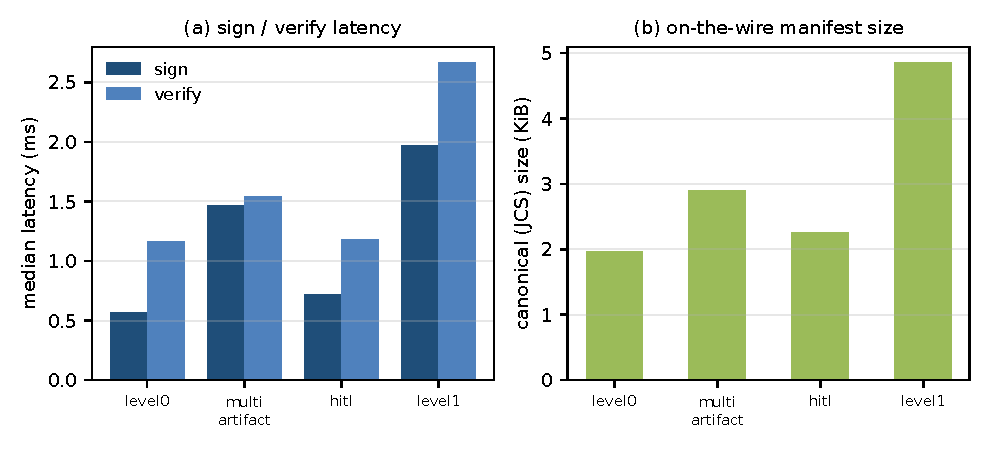
\includegraphics[width=\linewidth]{figures/sign_verify_size.pdf}
\caption{(a) Median Ed25519 sign and verify latency and (b) canonical (JCS) manifest
size across the committed example manifests. Generated by \texttt{experiments/plot.py}
from the measured \texttt{bench.json}.}
\label{fig:signsize}
\end{figure}

\paragraph{Delegation-chain scaling.}
We built signed delegation chains of depth 1 to 10 using the shipped
\texttt{DelegationHopSigner}, narrowing scope monotonically at each hop (dropping one
tool and decrementing the depth budget), and verified each chain with the shipped
\texttt{verify\_delegation\_chain}. Verification latency is close to linear in
chain depth (Figure~\ref{fig:deleg}): depths 1 to 9 cost about 0.21\,ms per hop
(0.21\,ms for one hop, 1.99\,ms for nine), and the ten-hop median, 2.96\,ms, sits
above that line.

\begin{figure}[h]
\centering
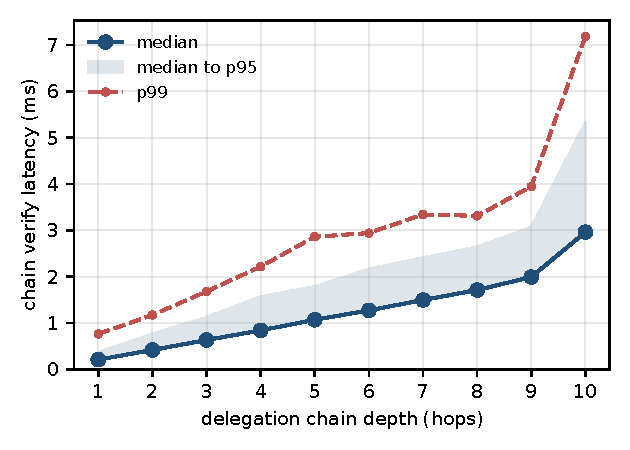
\includegraphics[width=0.62\linewidth]{figures/delegation_latency.pdf}
\caption{Delegation-chain verification latency versus chain depth (1 to 10 hops),
median with the median-to-p95 band and the p99 line. Each hop is signed by the shipped
\texttt{DelegationHopSigner} and verified by \texttt{verify\_delegation\_chain}.}
\label{fig:deleg}
\end{figure}

\paragraph{Tamper detection.}
Starting from a signed Level~1 manifest that verifies \texttt{VALID}, we mutated each
of ten bound fields in turn (six artifact fields, namely five digests and the model
version, plus \texttt{agent\_id}, \texttt{issuer}, \texttt{manifest\_id}, and
\texttt{issued\_at}) and re-verified without re-signing. In all ten cases
verification no longer returned \texttt{VALID}: the mutated canonical bytes fail the
single signature, so the tamper is caught (fail-closed). This shows that the
signature covers these fields. The probe supplies no runtime artifact digests, so
comparison against a deployed agent's artifacts is not exercised. The verifier at
this revision also did not recompute the declared tool-catalog root from the per-tool
entries: the committed Level~0 example declares a root that its own tool list does
not produce, verifies \texttt{VALID} here, and returns \texttt{MISMATCH} on current
SDK main.

\section{Related Work and Regulatory Mapping}
\label{sec:related}

\paragraph{Standards composition.}
Agent Manifest composes rather than replaces. It reuses SPIFFE~\citep{spiffe2018} for
identity, RFC~8785~\citep{jcs8785} for canonicalization, Ed25519~\citep{eddsa8032} and
ML-DSA-65~\citep{mldsa204} for signatures, RFC~9162~\citep{ct9162} Merkle trees and
Sigstore/Rekor~\citep{sigstore2021} for transparency, SLSA~\citep{slsa2023} and
SBOM formats for supply-chain provenance, RATS/EAT~\citep{rats2021,eat2023} for
attestation, and UUIDv7~\citep{uuid9562} for identifiers. Its contribution is the
\emph{binding rule} that places each of these into one signed, hardware-attestable
record scoped to an agent.

\paragraph{Relative to the runtime stack.}
Static documentation (model cards, AIBOMs) describes intent but is unbound to what
deployed; runtime governance frameworks enforce behavior but do not attest identity
and provenance; platform attestation proves the environment but not the agent. Agent
Manifest is the identity-and-provenance layer that the runtime evidence formats
(TRACE and cMCP~\citep{trace2026,cmcp2026}) and governance toolkits like
AGT~\citep{agt2026} build on.

\paragraph{Regulatory mapping.}
The manifest's records map onto emerging obligations: tamper-evident record-keeping
for high-risk AI (EU AI Act Article~12) is served by the signed, transparency-anchored
manifest; human-oversight requirements (Article~14)~\citep{euaiact2024} by the HITL
record (Section~\ref{sec:deleg}); and equivalent audit-trail duties under sector
regimes (financial, healthcare) by the same evidence. Agent Manifest does not claim
compliance; it produces the cryptographic evidence a compliance program needs.

\section{Conclusion}
\label{sec:conclusion}

Agent Manifest gives an AI agent a verifiable identity. By binding the ten artifacts
that define an agent (system prompt, policy, tools, model, retrieval corpus,
memory, decision trace, delegation, supply chain, and human approvals) into one
signed, hardware-attestable, tamper-evident record, it lets a verifier detect differences between supplied artifacts and a signed
baseline. Establishing that those artifacts were used in a deployed agent requires
additional runtime evidence and trusted attestation binding. The design favors
tamper-evidence over tamper-resistance, reuses established primitives (SPIFFE, JCS,
Ed25519/ML-DSA, RFC~9162 Merkle trees, RATS/EAT), and slots into the runtime stack
alongside cMCP and TRACE for attestation and AGT for policy.

\paragraph{Limitations and future work.}
The format is settled for the static artifacts; several pieces are staged. Memory and
retrieval bindings capture a baseline and a drift policy but continuous in-flight
verification of mutating state is future work. The post-quantum profile is specified
and implemented but was not exercised: its tests skip without the ML-DSA
dependency. Federated, cross-organization
verification (where one trust domain appraises another's manifests) is targeted
for the next revision, alongside richer multi-model manifests. The specification is a
developer-preview draft; the roadmap is community hardening toward an open standard
with multiple independent implementations and conformance certification.


\bibliographystyle{plainnat}
\bibliography{refs}

\end{document}
